\section{Product perspective}
% here we include further details on the shared phenomena and a domain model (class diagrams and statecharts)

The application will offer some services based on data gathered from individuals. In particular, the three services are the following:

\begin{itemize}
    \item The \emph{Data4Help} service has as the main goal of providing user data to Third-parties, allowing them to know their position and health status.
    To do that, the Individuals have to collect their data through smart-watches and allow the system to store them. Upon successful requests, the system provides Third-parties with the already collected data and will send the new data according to the frequency of updates and granularity specified during the request compilation, if a subscription is performed.
    At any time, Third-parties can unsubscribe, in this way they won't receive updates but but they can still access already gathered data, relative to past requests.
    \item The \emph{AutomatedSOS} service has as the main goal of offering an SOS service to Elderly people. To do that, the system accepts Elderly people subscriptions in order to collect and analyses data gathered by their \emph{Data4Help} account. In case of critical health values, the system sends the exact position to the ambulance service, in order to send an ambulance to the rescue.
    \item The \emph{Track4Run} service has as the main goal of organising runs. The system allows organisers to define all details of a run: path, starting date and time, maximum number of participants. After the creation of a run, people registered to \emph{Data4Help} service can enrol to the race simply through their D4H account. In order to not exceed the maximum participants number, the software keeps track of the number of runners already enrolled. During the competition, everyone ( an account is not needed ) can monitor on a map the exact position of all runners; at the end of the race, the system stores the rankings to make it available in the future to both participants and organisers. 
\end{itemize}


\begin{figure}[H]
    \centering
    \makebox[\textwidth][c]{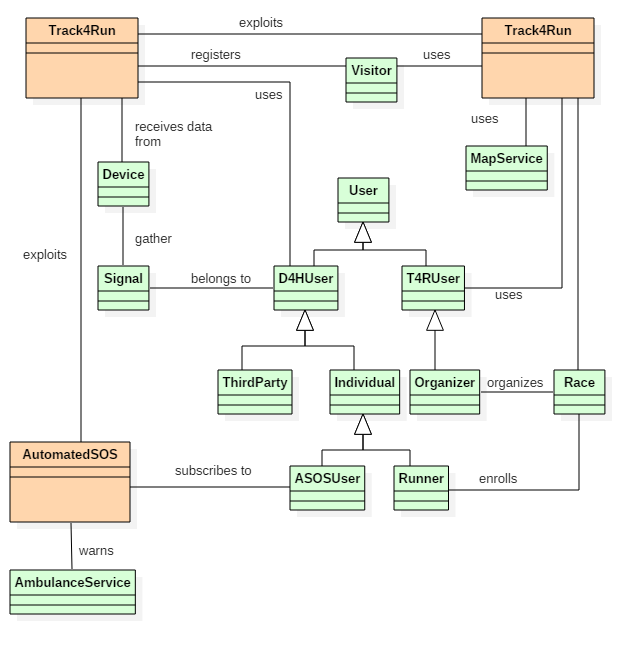
\includegraphics[scale=0.75]{./pictures/ClassDiagram2.png}}
    \caption{Class diagram of the entire system}
    \label{fig:class-diagram}
\end{figure}